\section{Efficient Training at Scale}
\label{sec:train}

In the realm of LLMs, efficient training at scale becomes paramount. As we venture into deeper and more expansive models, the computational demands surge explosively. Handling such computation requirements without compromising on model accuracy necessitates the adoption of state-of-the-art algorithmic optimizations, communication strategies, data pipeline management, and network performance tuning techniques. This section delves deep into the methods employed to optimize the training of large models in order to achieve high training efficiency at scale.

\subsection{Algorithmic Optimizations}
\label{sec:algorithm}

We make a few modifications and incorporate recent optimizations at
the algorithmic level to improve training efficiency, without compromising
accuracy. We validate
the impact of these techniques on model convergence in~\S\ref{sec:experience:covergence}.


\parabf{Parallel transformer block~\cite{gpt-j}.} We adopt a parallel version of the transformer block in lieu of the standard serialized formulation. 
Specifically, the standard formula of the transformer block can be reformatted from 
\begin{equation}
    \begin{aligned}
        y = x + \text{MLP}(\text{LN}(x + \text{Attention}(\text{LN}(x))))
    \end{aligned}
\end{equation}
into
\begin{equation}
    \begin{aligned}
        y = x + \text{MLP}(\text{LN}(x)) + \text{Attention}(\text{LN}(x))
    \end{aligned}
\end{equation}

With this approach, the computation of the attention block and the MLP block can
be executed in parallel, thereby reducing the computation time. Prior
work~\cite{chowdhery2022palm} shows that this modification does not degrade the
quality of models with parameters in the hundreds of billions.


\begin{figure*}[t!]
    \centering
     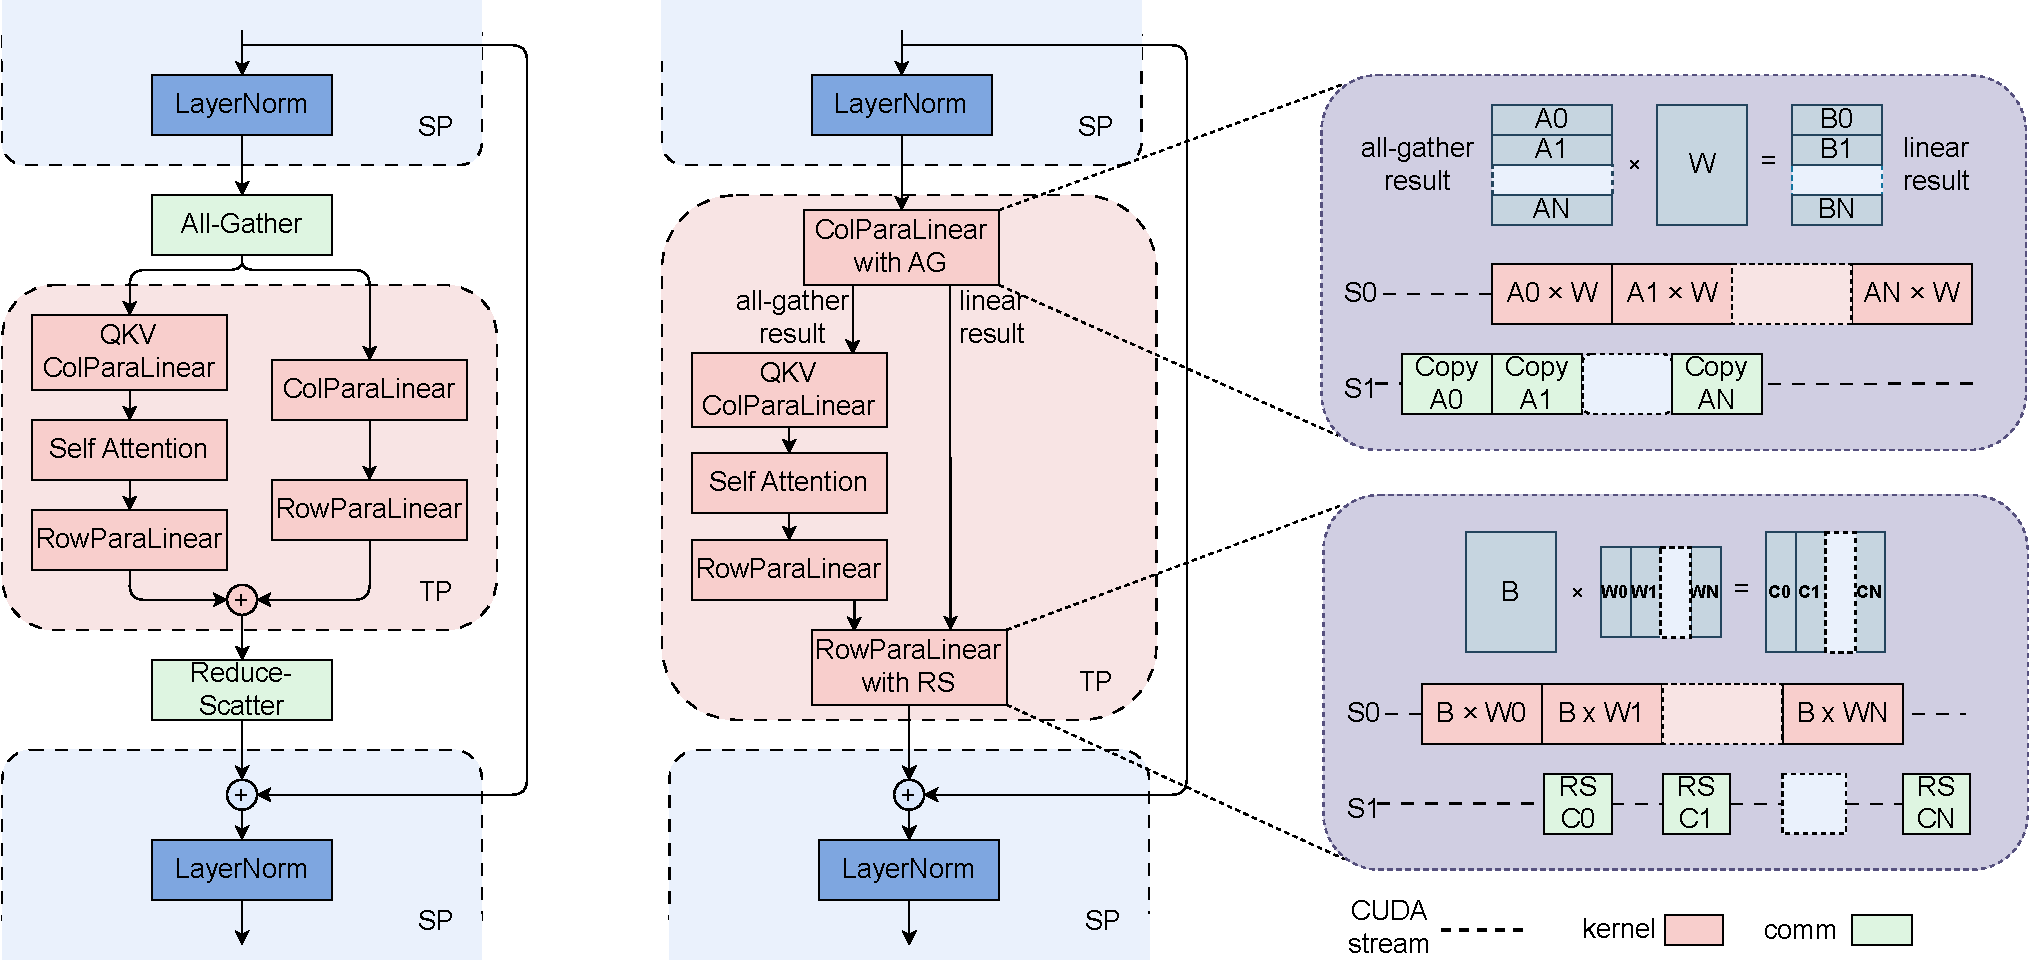
\includegraphics[width=0.96\textwidth]{figures/tp-overlap/ptb-combined.pdf}
     % \vspace{-0.1in}
     \\
     (a) PTB with SP and TP \hspace*{0.6in} (b) Fuse communication into Linears \hspace*{0.4in} (c) Overlap communication with GEMM
     \caption{Overlapping communication in tensor parallelism (TP) and sequence parallelism (SP) with parallel transformer block (PTB).}
    \label{fig:ptb}
\end{figure*}

\parabf{Sliding window attention (SWA)}. Sliding window
attention~\cite{beltagy2020longformer} is a sparse attention mechanism that
employs a fixed-size window surrounding each token in the input sequence. The
computation complexity is $O(s \times w)$, where $s$ is the input sequence
length and $w$ is the fixed window size. Sliding window attention is more
efficient than the full self-attention, whose computation complexity is $O(s
\times s)$, given that $w\ll s$. \revision{Past work~\cite{beltagy2020longformer} and our micro-benchmark (\S\ref{sec:experience:covergence}) have shown that} 
the information across the entire input can be retained with a large receptive
field created by stacking layers of such windowed attention. This enables faster training without compromising the accuracy.


\parabf{LAMB optimizer}. Efficient training at a large scale is often
hindered by batch size constraints. Particularly, increasing the batch size may
adversely affect model convergence. The LAMB optimizer~\cite{You2020Large} has been
demonstrated to enable the scaling of BERT's training batch size to 64K without
compromising accuracy. In the LLM setting, our experiments find that LAMB
can scale the batch size to 4$\times$ without accuracy loss. With
interleaved pipeline parallelism, the original schedule contains $\frac{4}{v}
\frac{p-1}{m}$ pipeline bubbles when training four steps with 1$\times$ batch
size~\cite{narayanan2021efficient}, while the pipeline bubbles of training one
step with 4$\times$ batch size are $\frac{1}{v} \frac{p-1}{4m}$. Hence, {\sysname}
reduces 87.5\% of the pipeline bubbles via LAMB optimizer. 



\subsection{Communication Overlapping in 3D Parallelism}
\label{sec:overlap}


To reduce the iteration time, we systematically analyze the dependencies between
computation and communication for all the operators in 3D parallelism, and
design techniques to hide the overhead of all the off-the-critical-path
operations.


\parabf{Overlapping in data parallelism.} 
As shown in Figure~\ref{fig:dp-zero}, for data parallelism, two main
communication operations stand out. One is the \textit{all-gather} operation,
which fetches the most recent model parameters from workers in other data
parallel ranks during the forward pass. The other is the \textit{reduce-scatter}
operation, which collect the gradients in the backward pass. In 3D parallelism,
a single device may host multiple model chunks. Overlapping is implemented on a
model chunk basis to maximize bandwidth utilization. The \textit{all-gather}
operation is triggered prior to the forward pass of a model chunk, and the
\textit{reduce-scatter} operation commences after its backward pass. This
results in a challenge where the first \textit{all-gather} operation and the
last \textit{reduce-scatter} operation cannot be hidden. Inspired by PyTorch
FSDP~\cite{pytorch_fsdp}, the initial \textit{all-gather} operation is
pre-fetched at the beginning of each iteration, allowing it to overlap with data
loading operations, effectively reducing the communication time by a factor of
$1/(2*vpp\_size)$.
We also launch the high priority communication first to maximize overlapping. The priorities of communication operators are determined by the order of the corresponding computation operators that depend on the communication result. 


\parabf{Overlapping in pipeline parallelism.} Pipeline parallelism features point-to-point \textit{send/receive} communication. \sysname uses the interleaved 1F1B scheduling method mentioned in~\ref{sec:background}. We note that in the warm-up phase, the forward pass only depends on its previous \textit{receive}. We thus decouple the \textit{send} and \textit{receive}, which are often implemented together and can be blocked by the slower one. By breaking this dependency, we enable the send operation to overlap with the computation as shown in the left part of Figure~\ref{fig:pp-overlap}. The cool-down phase can be viewed as the inverse of the warm-up phase, allowing for the inverse application of the same technique. As for the steady phase, both the forward and backward computation are independent of adjacent communication operations. Taking the backward as an example, as shown in the right part of Figure~\ref{fig:pp-overlap}, its previous \textit{receive} is for the next forward computation while the \textit{send} is for the backward computation in the previous stage. So the \textit{send} and \textit{receive} operations can be launched asynchronously to overlap with the computation.


\iffalse
\begin{figure*}
    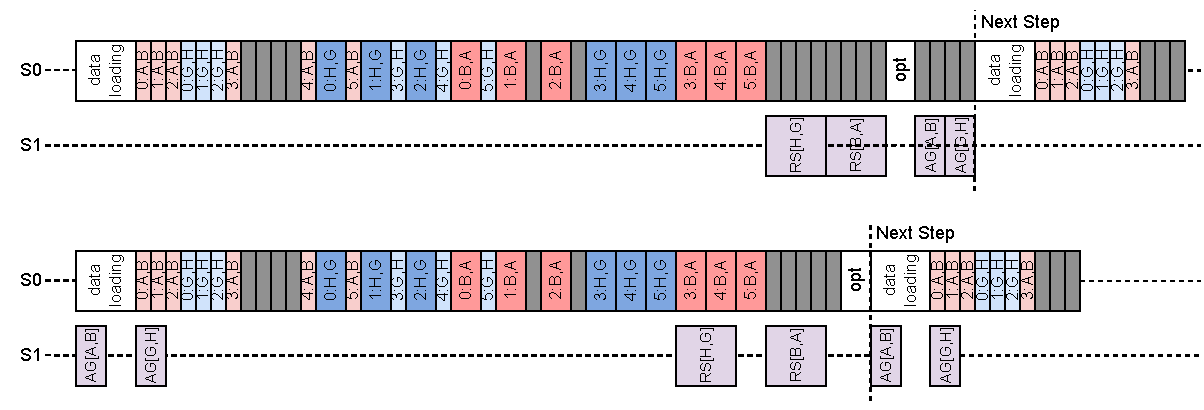
\includegraphics[width=0.98\textwidth]{figures/dp-overlap/dp-overlap.pdf}
    \caption{DP Overlap.}
    \label{fig:dp-overlap}
\end{figure*}
\fi


\begin{figure}[t]
    \centering
     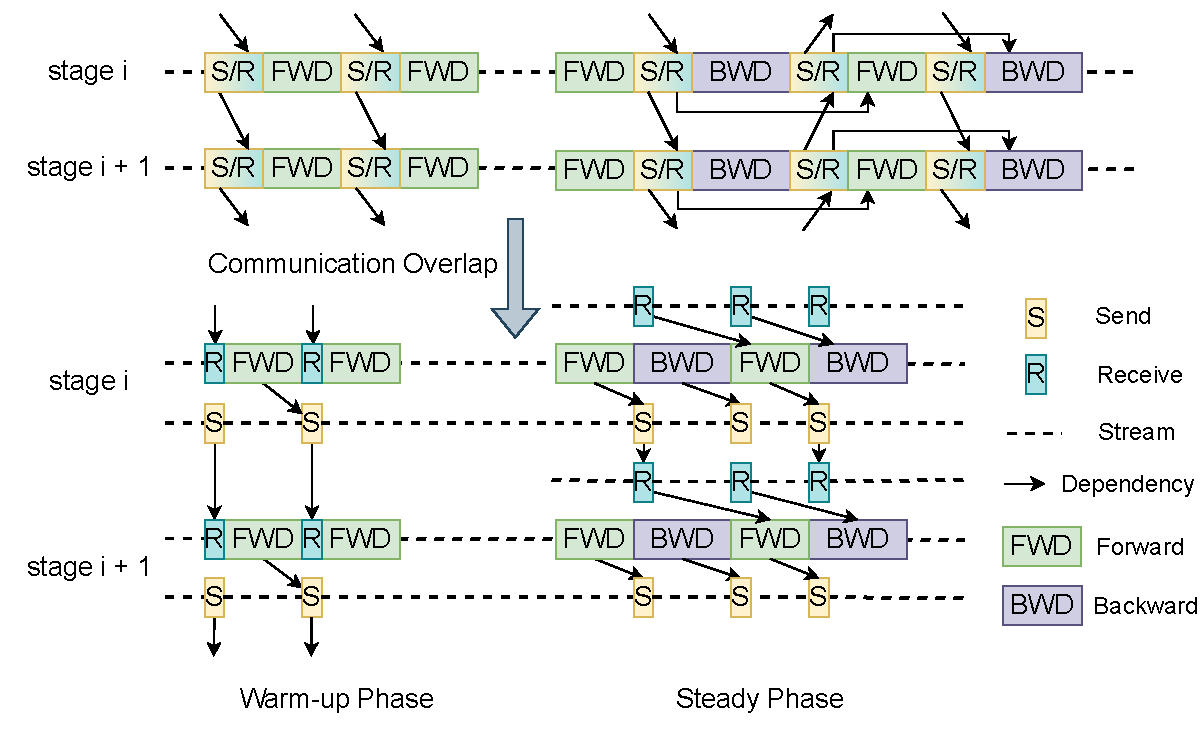
\includegraphics[width=0.46\textwidth]{figures/pp-overlap/pp-overlap.pdf}
     % \vspace{-0.1in}
     \hfill
     % (a)PTB with SP and TP \hspace*{0.6in} (b) Fuse communication into FFN \hspace*{0.4in} (c) Overlap communication with GEMM
     \caption{Overlapping communication in pipeline parallelism.}
    \label{fig:pp-overlap}
\end{figure}

\parabf{Overlapping in tensor/sequence parallelism.} Tensor parallelism is commonly used to partition weights in computational-intensive operations, while operations like \textit{LayerNorm} and \textit{Dropout} are partitioned along the sequence dimension to save GPU memory. This necessitates \textit{all-gather} and \textit{reduce-scatter} operations for input collection and output redistribution across GPUs. Figure~\ref{fig:ptb}\textcolor{green!80!black}{a} shows this communication pattern in the parallel transformer block architecture. Here the two communication operators are in the critical path. To eliminate this overhead, we choose to fuse \textit{all-gather} and \textit{reduce-scatter} with the parallel \textit{Linears} on the FFN path (Figure \ref{fig:ptb}\textcolor{green!80!black}{b}). Since the GEMM kernels on the FFN
path is larger, the communication can be hidden better. We break the GEMM kernel into small chunks, and pipeline the execution with the communication (Figure~\ref{fig:ptb}\textcolor{green!80!black}{c}). 
This strategy can be applied in the backward pass similarly.



\subsection{Efficient Operators}

Despite the optimization for GEMM operators in Megatron-LM, we identify
opportunities for further enhancement in other operators. For the attention part,
we adopt FlashAttention-2~\cite{dao2023flashattention}, which improves
work partitioning between different thread blocks and warps. For LayerNorm and GeLU, we observe that they
are composed of fine-grained kernels in previous implementations. By fusing
these kernels together, we reduce the overhead associated with launching
multiple kernels and aid in optimizing memory access patterns, thereby
achieving better performance.


\subsection{Data Pipeline}
\label{sec:data}

Data preprocessing and loading are often overlooked. However, these operations
create non-negligible GPU idle time at the beginning of each training step.
Optimizing these operations are essential for efficiency of the training
process.

\parabf{Asynchronous data preprocessing.} Data preprocessing is not on the
critical path. As a result, while the GPU workers are synchronizing gradients at
the end of each training step, the data preprocessing for the subsequent step
can start, which hides the preprocessing overhead.


\parabf{Redundant dataloader elimination.} In a typical data loading phase of
distributed training, each GPU worker is equipped with its own data loader,
responsible for reading training data into the CPU memory before forwarding it
to the GPU. This leads to competition among workers for disk read bandwidth,
thereby creating a bottleneck. Notably, we observe that in the LLM training
setting, GPU workers within the same machine are in the same tensor parallel
group. Consequently, their inputs for each iteration are inherently identical.
Based on this observation, we adopt a two-layer tree-based approach.
We use a single, dedicated data loader on each machine to read the
training data into a piece of shared memory. Subsequently, each GPU worker is
responsible for copying the necessary data to its own GPU memory. This
eliminates redundant reads and significantly enhances the efficiency of data
transfer.


\subsection{Collective Communication Group Initialization}

In distributed training, the initialization phase involves the establishment of
NVIDIA Collective Communications Library (NCCL) communication groups among GPU
workers. Since this overhead is relatively negligible in small-scale scenarios,
\texttt{torch.distributed} is used by default. As the number of GPUs scales to
over ten thousand, the overhead introduced by naive implementations becomes
intolerable. \revision{We conduct experiments on the same AI cluster in \S\ref{sec:experience} and our empirical measurement indicates that the initialization time for Megatron-LM on 2,048 NVIDIA Ampere GPUs is approximately 1047 seconds.} While this may
appear relatively small compared to the training duration, it imposes a
significant hurdle to routine testing and iterative development (e.g., minor
code adjustments in hyperparameter tuning and debugging). It also hampers
the implementation of fast restart-and-recovery mechanisms.

\revision{To address this issue, we perform a detailed profiling of
\texttt{torch.distributed}~\cite{li2020pytorch}} and identify two primary causes of excessive
initialization time. The first issue resides in the synchronization step, where
each process is involved in a barrier operation at the end of initialization a
specific communication group. \revision{This barrier uses TCPStore, an inner distributed Key-Value Store implementation in Pytorch which
operates in a single-threaded, blocking read-write manner.} We replace TCPStore
with Redis, which is non-blocking and asynchronous. This reduces the
initialization time to 361 seconds on 2,048 GPUs. The second issue is related to
the incautious usage of global barriers. Each process executes a global barrier
after initializing its corresponding communication group. We carefully design
the order in which communication groups are initialized to minimize the need for
global barriers. This approach lowers the time complexity of the global barrier from $O(n^2)$ to $O(n)$. The initialization time is reduced to under 5 seconds on 2048 GPUs, and to under 30 seconds on more than 10,000 GPUs with those optimizations.

\subsection{Network Performance Tuning}

We analyze the traffic across machines in 3D parallelism and design techniques to improve network performance.

\parabf{Network topology.} Our datacenter network is built with high-performance
switches based on Broadcom Tomahawk 4 chips. The total bandwidth of each Tomahawk
chip is 25.6Tbps with 64$\times$400Gbps ports. Three layers of switches are
connected in a CLOS-like topology to connect more than 10,000 GPUs. For switches
at each layer, the bandwidth percentage between downlink and uplink is 1:1. That
is, 32 ports are used as downlink and 32 ports are used as uplink. The network
provides high bandwidth with a small diameter. Every node can communicate with
other nodes within a limited number of hops.   

\parabf{Reducing ECMP hashing conflicts.}
We carefully design the network topology and schedule network traffic to reduce ECMP hashing conflicts. First, at the
top-of-rack (ToR) switch level, one 400G downlink port is split into two 200G
downlink ports with specific AOC cables. The conflict
probability is reduced as the bandwidth of each uplink is double of that
of a downlink. Second, eight 200G NICs on the server
is connected to eight different switches in a multi-rail way. The number of GPU
servers connected by the same sets of ToR switches can reach 64. And we strategically schedule the data-intensive nodes from our training tasks to operate under the same Top of Rack (ToR) switch. This approach significantly reduces the number of switch hops required for communication and further reduce ECMP hashing conflicts probability.

\parabf{Congestion control.} \revision{In distributed training, all-to-all communication may lead to congestion and elevated levels of Priority Flow Control (PFC)\cite{PFCStandard} when employing the default DCQCN\cite{zhu2015congestion} protocol at scale. Excessive use of PFC can result in head-of-line (HoL) blocking \cite{zhu2015congestion}, thereby diminishing network throughput. To mitigate these issues, we have developed an algorithm incorporating principles from both Swift\cite{kumar2020swift} and DCQCN, which integrates the precise measurement of Round-Trip Time (RTT) with the rapid congestion response capabilities of Explicit Congestion Notification (ECN). This approach significantly enhances throughput and minimizes congestion related to PFC.}


\parabf{Retransmit timeout setting.} Parameters in NCCL can be set to control
retransmit timer and retry count. We tune these parameters for fast recovery under link
flapping.
To further reduce the recover time, we enable the adap\_retrans
feature on the NIC. This feature enables retransmission in a shorter interval
and help recover the transmission more quickly when the link flapping period is short.